\section{ELEMENT TACTICS}

\subsection{ELEMENT RESPONSIBILITIES}

\subsection{OFFENSIVE}

\begin{tcoloritemize}
    \blueitem[Notch-Press]
\end{tcoloritemize}

\begin{figure}[htbp]
    \centering
    \begin{tikzpicture}[figstyle]

        % coordinates
        \coordinate (naked_start) at (5,0);
        \coordinate (spiked_start) at (-5,0);
        \coordinate (bandit) at (0,70);

        \coordinate (naked_notch_start) at (5,25);
        \coordinate (spiked_notch_start) at (-5,25);

        % bandit wez
        \draw[fill=red!40]
            (bandit)
            -- ++(-110:48)
            arc (-110:-120:48)
            -- (bandit);

        \node[rotate=-90] (naked_notch_mid) at (20, 30) {
            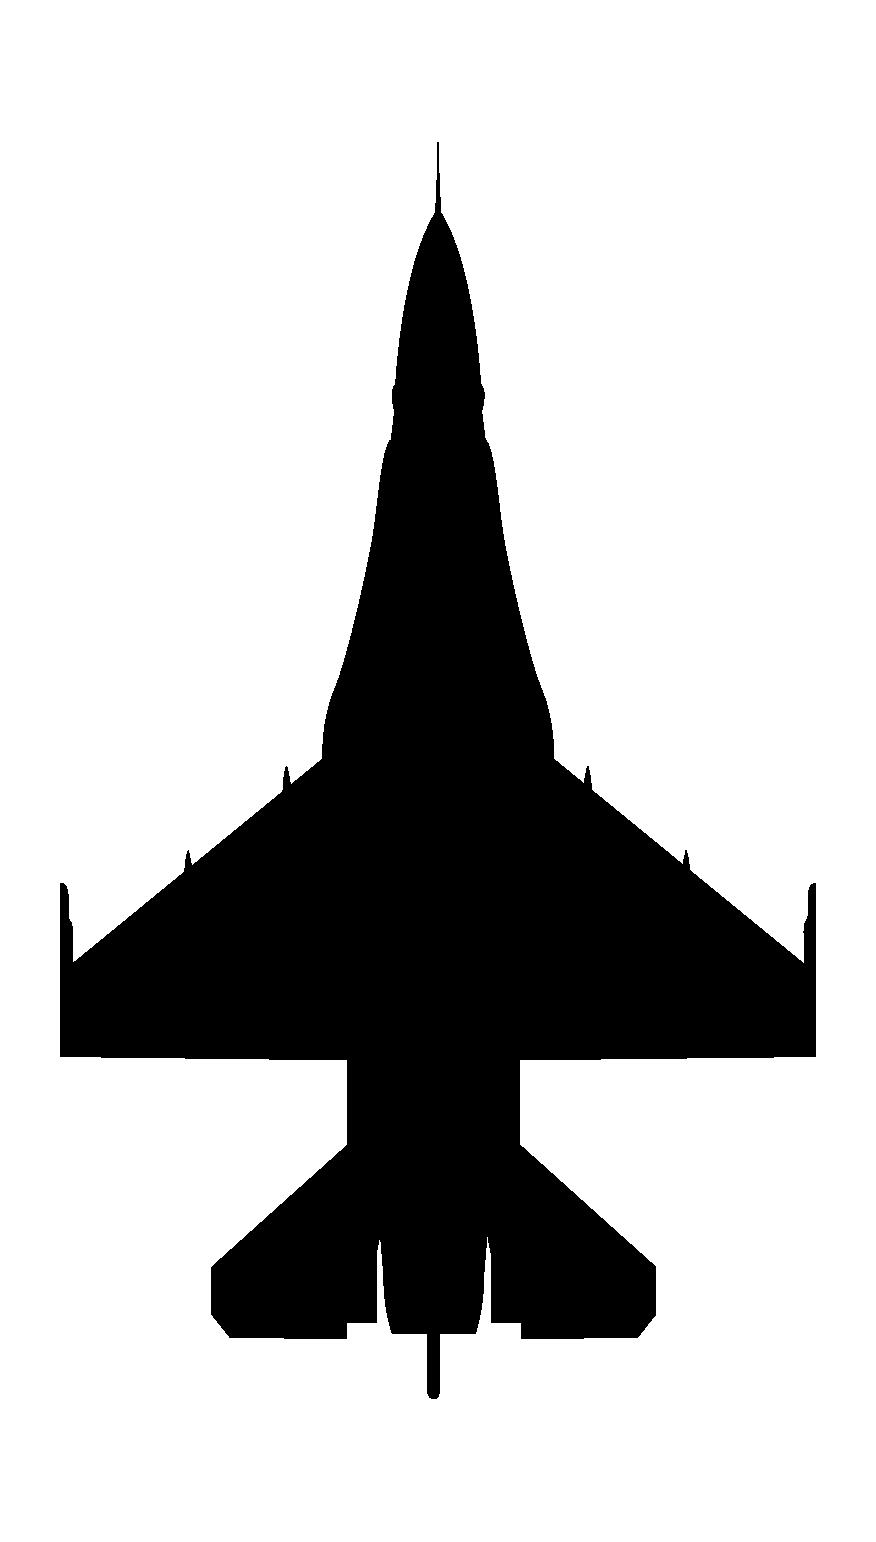
\includegraphics[
                width=7.5mm,
            ]{diagrams/aircraft/silhouette_f16_top.pdf}
        };
        \node[rotate=90] (spiked_notch_mid) at (-20, 30) {
            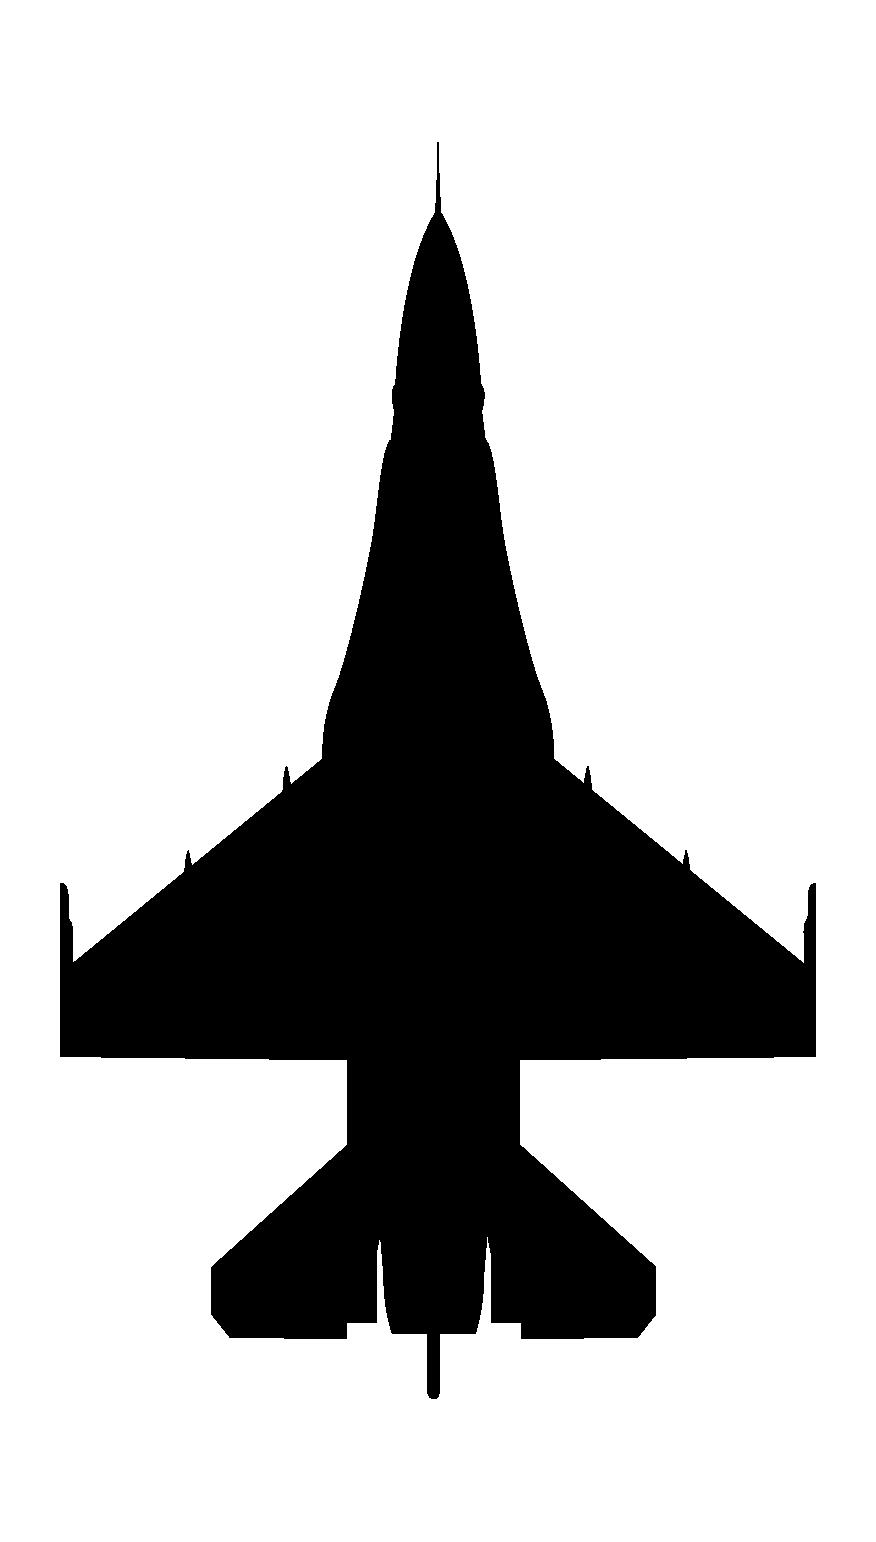
\includegraphics[
                width=7.5mm,
            ]{diagrams/aircraft/silhouette_f16_top.pdf}
        };
        
        % naked fighter
        \draw[->] 
            (naked_start) -- 
            node[below, pos=0]{
                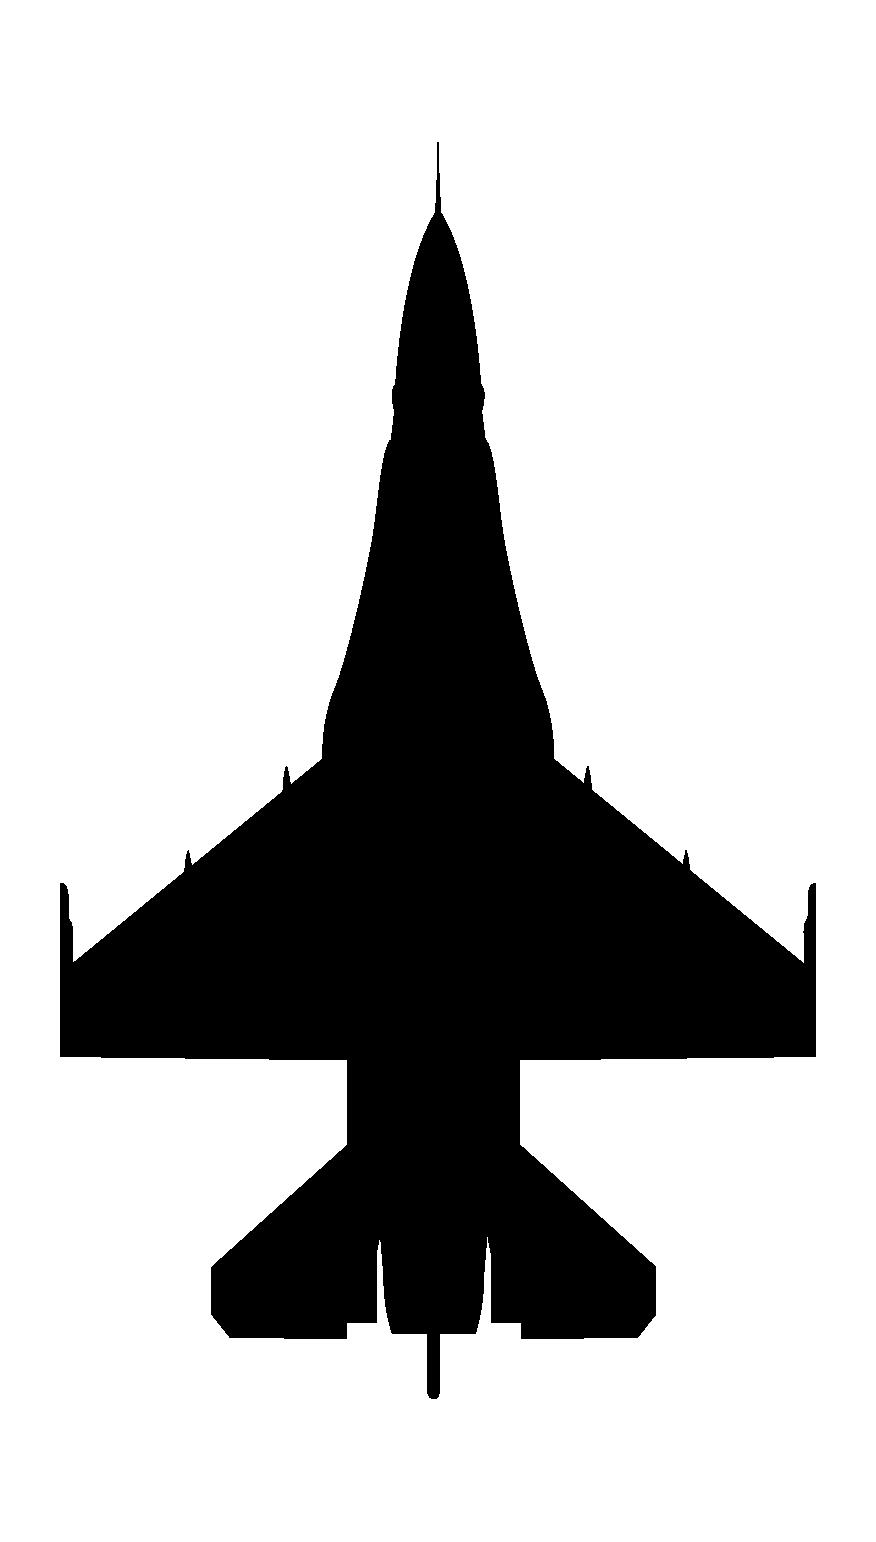
\includegraphics[
                width=7.5mm,
            ]{diagrams/aircraft/silhouette_f16_top.pdf}} 
            (naked_notch_start)
            arc (180:90:5) 
            -- (naked_notch_mid);
        \draw[->]
            (naked_notch_mid.north)
            arc (-90:45:5) 
            -- ++(135:10)
            node[above, pos=1, rotate=45] (naked_commit) {
                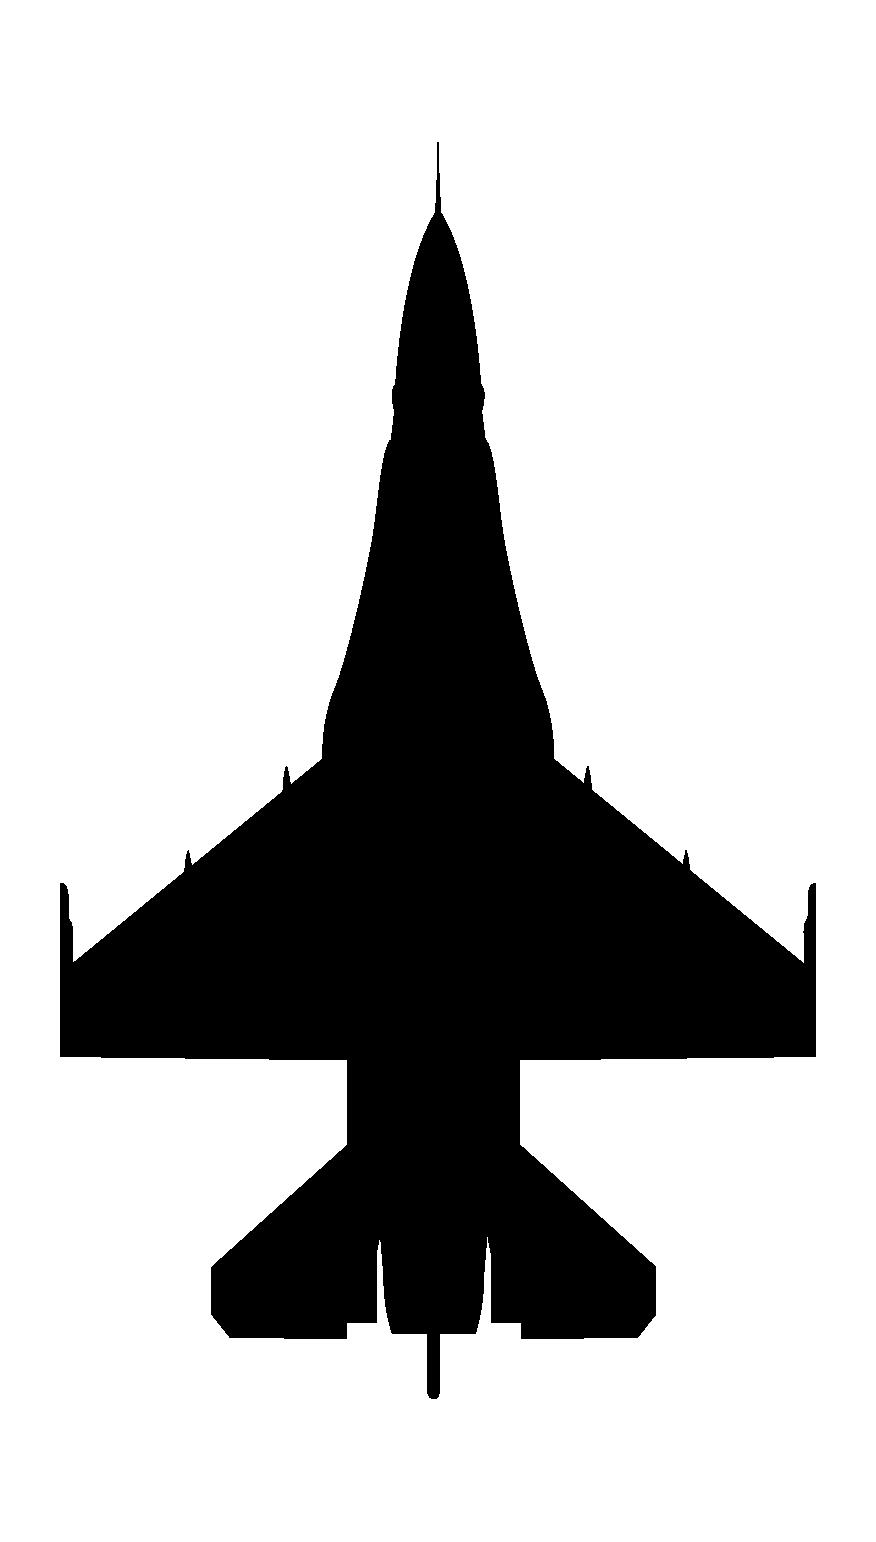
\includegraphics[
                    angle=0,
                    width=7.5mm,
            ]{diagrams/aircraft/silhouette_f16_top.pdf}};

        \node[font=\footnotesize, below] at (naked_notch_mid.east) {Naked}; 
        \node[font=\footnotesize, right] at (naked_commit.east) {Commit};

        % spiked fighter
        \draw[->] 
            (spiked_start) -- 
            node[below, pos=0]{
                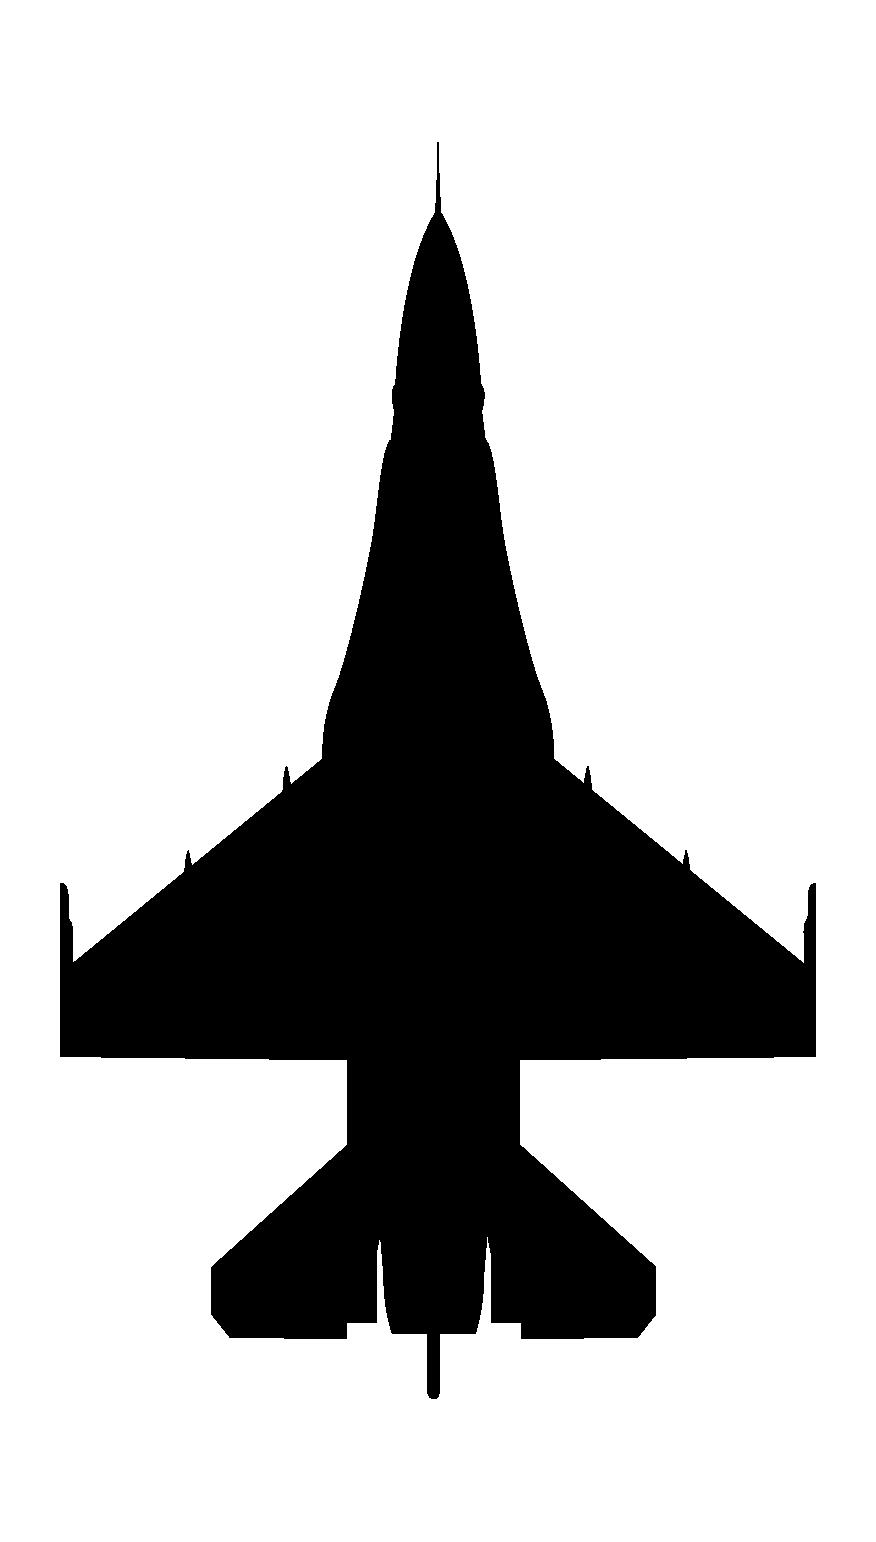
\includegraphics[
                width=7.5mm,
            ]{diagrams/aircraft/silhouette_f16_top.pdf}} 
            (spiked_notch_start)
            arc (0:90:5) 
            -- (spiked_notch_mid);
        \draw[->]
            (spiked_notch_mid.north)
            arc (90:180:5) 
            -- ++(0,-10)
            node[below, pos=1] (spiked_abort) {
                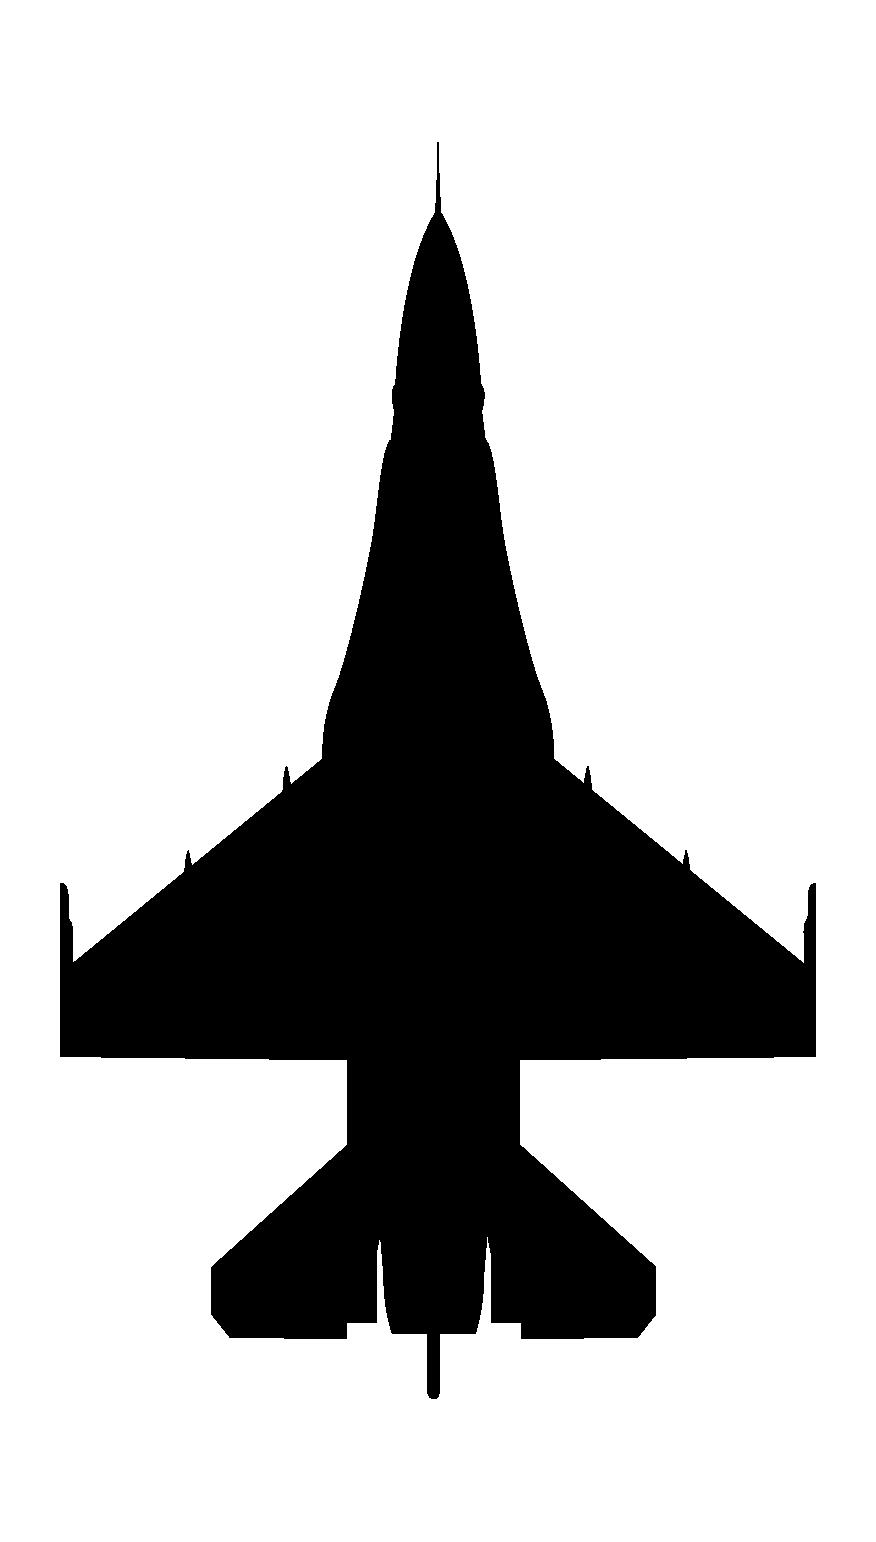
\includegraphics[
                    angle=180,
                    width=7.5mm,
            ]{diagrams/aircraft/silhouette_f16_top.pdf}};

        \node[font=\footnotesize, below] at (spiked_notch_mid.west) {Spiked}; 
        \node[font=\footnotesize, below] at (spiked_abort.south) {Abort};

        % bandit
        \node[] at (bandit) {
            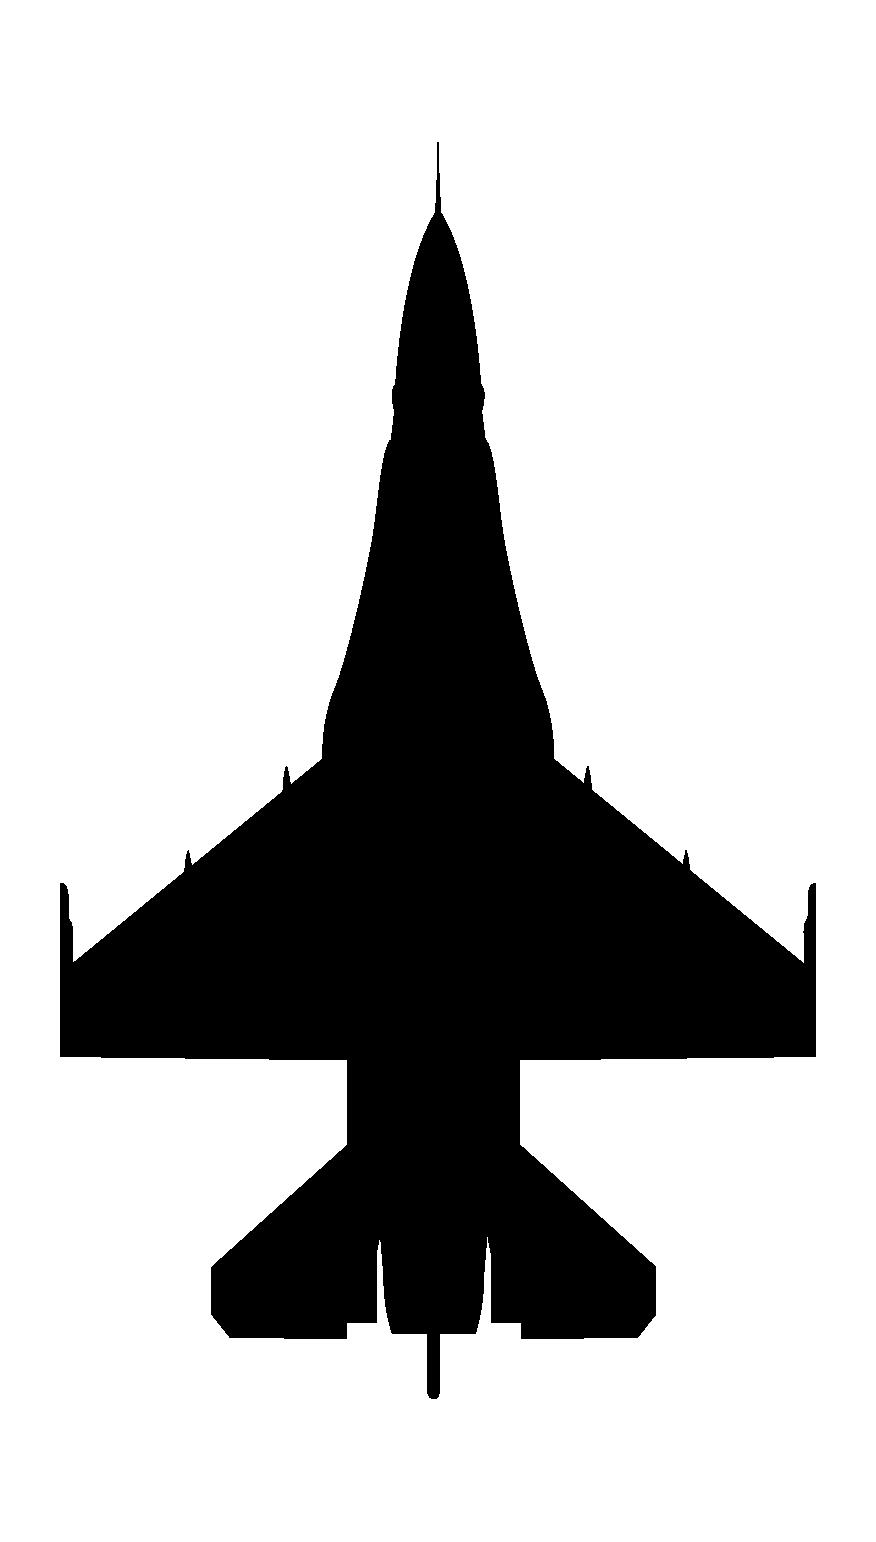
\includegraphics[
                angle=180,
                width=7.5mm,
        ]{diagrams/aircraft/silhouette_f16_top.pdf}};

    \end{tikzpicture}
    \caption{Notch-press tactics}
    \label{fig:ttp_aa:element:offensive:notchpress}
\end{figure}

\subsection{DEFENSIVE}

\begin{tcoloritemize}
    \blueitem[Stagger-Back]
    \blueitem[Notch-Back]
\end{tcoloritemize}